\begin{figure}[h]
  \centering
  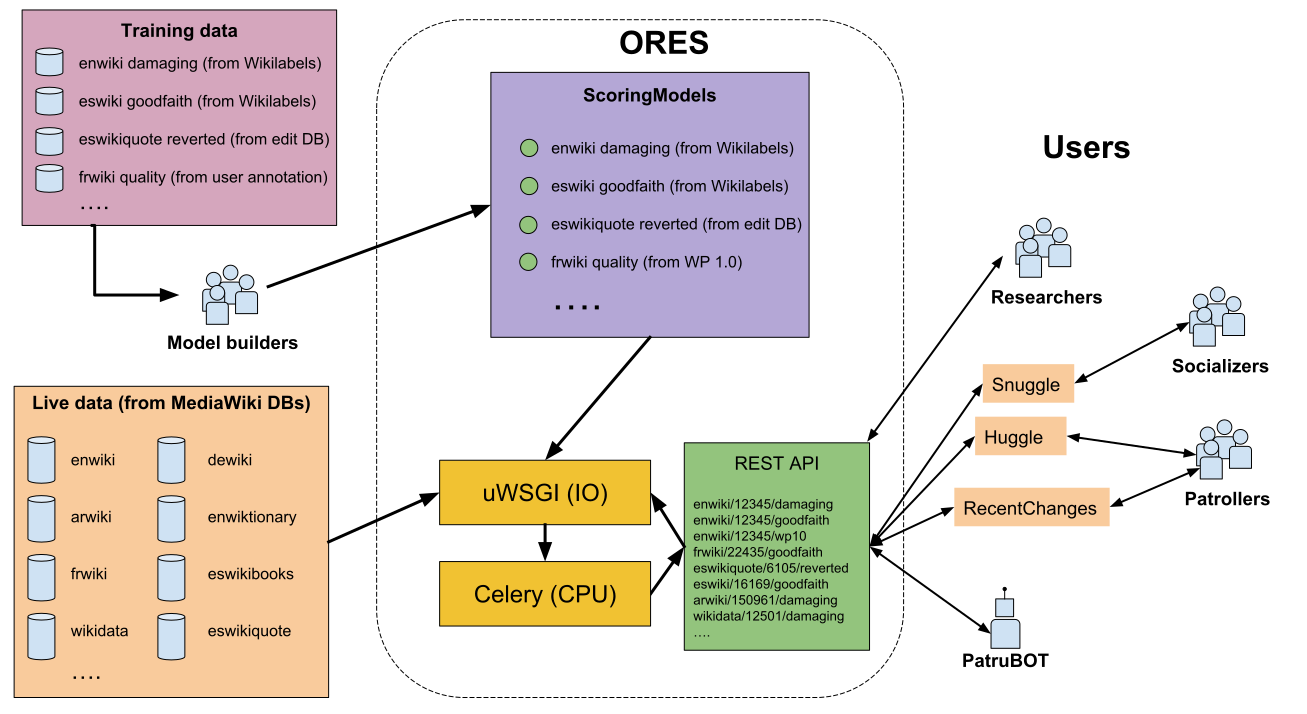
\includegraphics[width=.95\textwidth]{figures/ores_data_user_diagram}
  \caption{ORES conceptual overview.  Model builders design process for training ScoringModels from training data.  ORES hosts ScoringModels and makes them available to researchers and tool developers.}
  \label{fig:ores_data_user}
\end{figure}

ORES has been iteratively engineered to meet the needs of Wikipedia editors and the tools that support their work.  In this section, we describe the architecture of the system and how architecutral decisions allowed ORES to be intergrated into different types of workflows.

\subsection{Conceptual architecture}
At the core, ORES is a collection of machine classifier models and an API.  These models are designed and engineered by a varied set of model builders (some external researchers and others by our own research team) using varied sources of \emph{training data}.  The models that ORES hosts are engineered to support Wikipedian processes related to damage-detection, quality-assessment, and topic-routing, but the system is adaptable to a wide range of other models.

To make these models available for user, ORES implements a simple container service where the ``container'', referred to as a \emph{ScoringModel}, represents a fully trained and tested prediction model.  All \emph{ScoringModels} contain metadata about when the model was train/tested and which features are necessary for making a prediction.  All predictions take the form of a JSON document.  The ORES service provides access to ScoringModels via via a RESTful HTTP interface and serves the predictions (JSON documents) to users.  We chose this service structure because Wikimedian tool developers (our target audience) are familiar with this RESTful API/JSON workflow due to the dominant use of the MediaWiki API among tool developers.

\subsection{Scaling \& robustness}
To be useful for Wikipedians and tool developers, ORES uses distributed computation strategies to provide a robust, fast, high-availability service.  Reliability is a critical concern in Wikipedian quality control work.  Interruptions in Wikipedia's algorithmic systems have historically led to increased burdens for human workers and a higher likelihood that readers will see vandalism\cite{geiger2013levee}.  As previously discussed, we wanted to support Wikipedians who did not have the access and ability to operate a machine learning classifier at datacenter scales. The widespread use of ORES for multiple models across language versions of Wikimedia wikis could potentially involve orders of magnitude more computation than has ever been used for machine learning in Wikipedia.

This horizontal scaleability is achieved in two ways: input-output (IO) workers (uwsgi\footnote{\url{https://uwsgi-docs.readthedocs.io/}}) and the computation (CPU) workers (celery\footnote{\url{http://www.celeryproject.org/}}).  Requests are split across available IO workers, and all necessary data is gathered using external APIs (e.g. the MediaWiki API\footnote{\url{http://enwp.org/:mw:MW:API}}).  The data is then split into a job queue managed by \emph{celery} for the CPU-intensive work.  This efficiently uses available resources and can dynamically scale, adding and removing new IO and CPU workers in multiple datacenters as needed.  This is also fault-tolerant, as servers can fail without failing the service as a whole.

\subsection{Real-time processing}
The most common use case of ORES is real-time processing of edits.  For example, those using counter-vandalism tools like Huggle monitor edits within seconds of when they are made.  It is critical that ORES return these requests return in a timely manner.  We implement several strategies to optimize this request pattern.

\leadin{Single score speed}
In the worst case scenario, ORES is generating a score from scratch.  This is the common case when a score is requested in real-time---which invariably occurs right after the target edit or article is saved.  We work to ensure that the median score duration is around 1 second.  Our metrics tracking currently suggests that for the week April 6-13th, our median, 75\%, and 95\% score response timings are 1.1, 1.2, and 1.9 seconds respectively.

\leadin{Caching and precaching}
In order to take advantage of our users' overlapping interests in scoring recent activity, we also maintain a basic least-recently-used (LRU) cache\footnote{Implemented natively by Redis, \url{https://redis.io}} using a deterministic score naming scheme (e.g. \texttt{enwiki:123456:damaging} would represent a score needed for the English Wikipedia damaging model for the edit identified by 123456).  This allows requests for scores that have recently been generated to be returned within about 50ms via HTTPS.  In other words, a request for a recent edit that had previously been scored is 20X faster due to this cache.

In order to make sure that scores for \emph{all recent edits} are available in the cache for real-time use cases, we implement a ``precaching'' strategy that listens to a high-speed stream of recent activity in Wikipedia and automatically requests scores for a specific subset of actions (e.g. edits).  With our LRU and pre-caching strategy, we attain a cache hit rate of about 80\% consistently.

\leadin{De-duplication}
In real-time ORES use cases, it's common to receive many requests to score the same edit/article right after it was saved.  We use the same deterministic score naming scheme from the cache to identify scoring tasks, and ensure that simultaneous requests for that same score attach to the same result (or pending result) rather that starting a duplicate scoring job.  This pattern is very advantageous in the case of precaching, because of our network latency advantage: we can generally guarantee that the precaching request for a specific score precedes the external request for a score.  All waiting requests attach to the result of a single score generation process that starts prior to receiving the external request.  So even in worst-case scenarios where we're still calculating scores, we often see a better-than-expected response speed from the tool user's point of view.

\subsection{Batch processing}
Many different types of Wikipedia's bots rely on batch processing strategies to support Wikipedian work processes\cite{geiger2011lives}, so ORES needs to support sudden, high-intensity querying.  For example, many bots are designed to build worklists for Wikipedia editors (e.g. \cite{cosley2007suggestbot}) and recently, many of them have adopted ORES to include an article quality prediction for use in prioritization (see section~\ref{sec:adoption_patterns}).  Work lists are either built from the sum total of all 5m+ articles in Wikipedia, or from some large subset specific to a single WikiProject (e.g. WikiProject Women Scientists claims about 6k articles\footnote{As demonstrated by \url{https://quarry.wmflabs.org/query/14033}}.).  We've observed robots submitting large batch processing jobs to ORES once per day.  It's relevant to note that many researchers are also making use of ORES for various analyses, and their activity usually shows up in our logs as a similar burst of requests.

In order to most efficiently support this type of querying activity, we implemented batch optimizations in ORES by splitting IO and CPU operations into distinct stages.  During the IO stage, all data is gathered to generate a set of scores.  During the CPU stage, scoring jobs are split across our distributed processing system.  This batch processing affords up to a 5X increase in time to scoring speed for large requests\cite{sarabadani2017building}.  At this rate, a user can score 1 million revisions in less than 24 hours in the worst case scenario (no scores were cached)---which is unlikely for recent Wikipedia activity.

\subsection{Empirical access patterns}
\begin{figure*}[h]
\centering
\begin{subfigure}[t]{\textwidth}
  \centering
  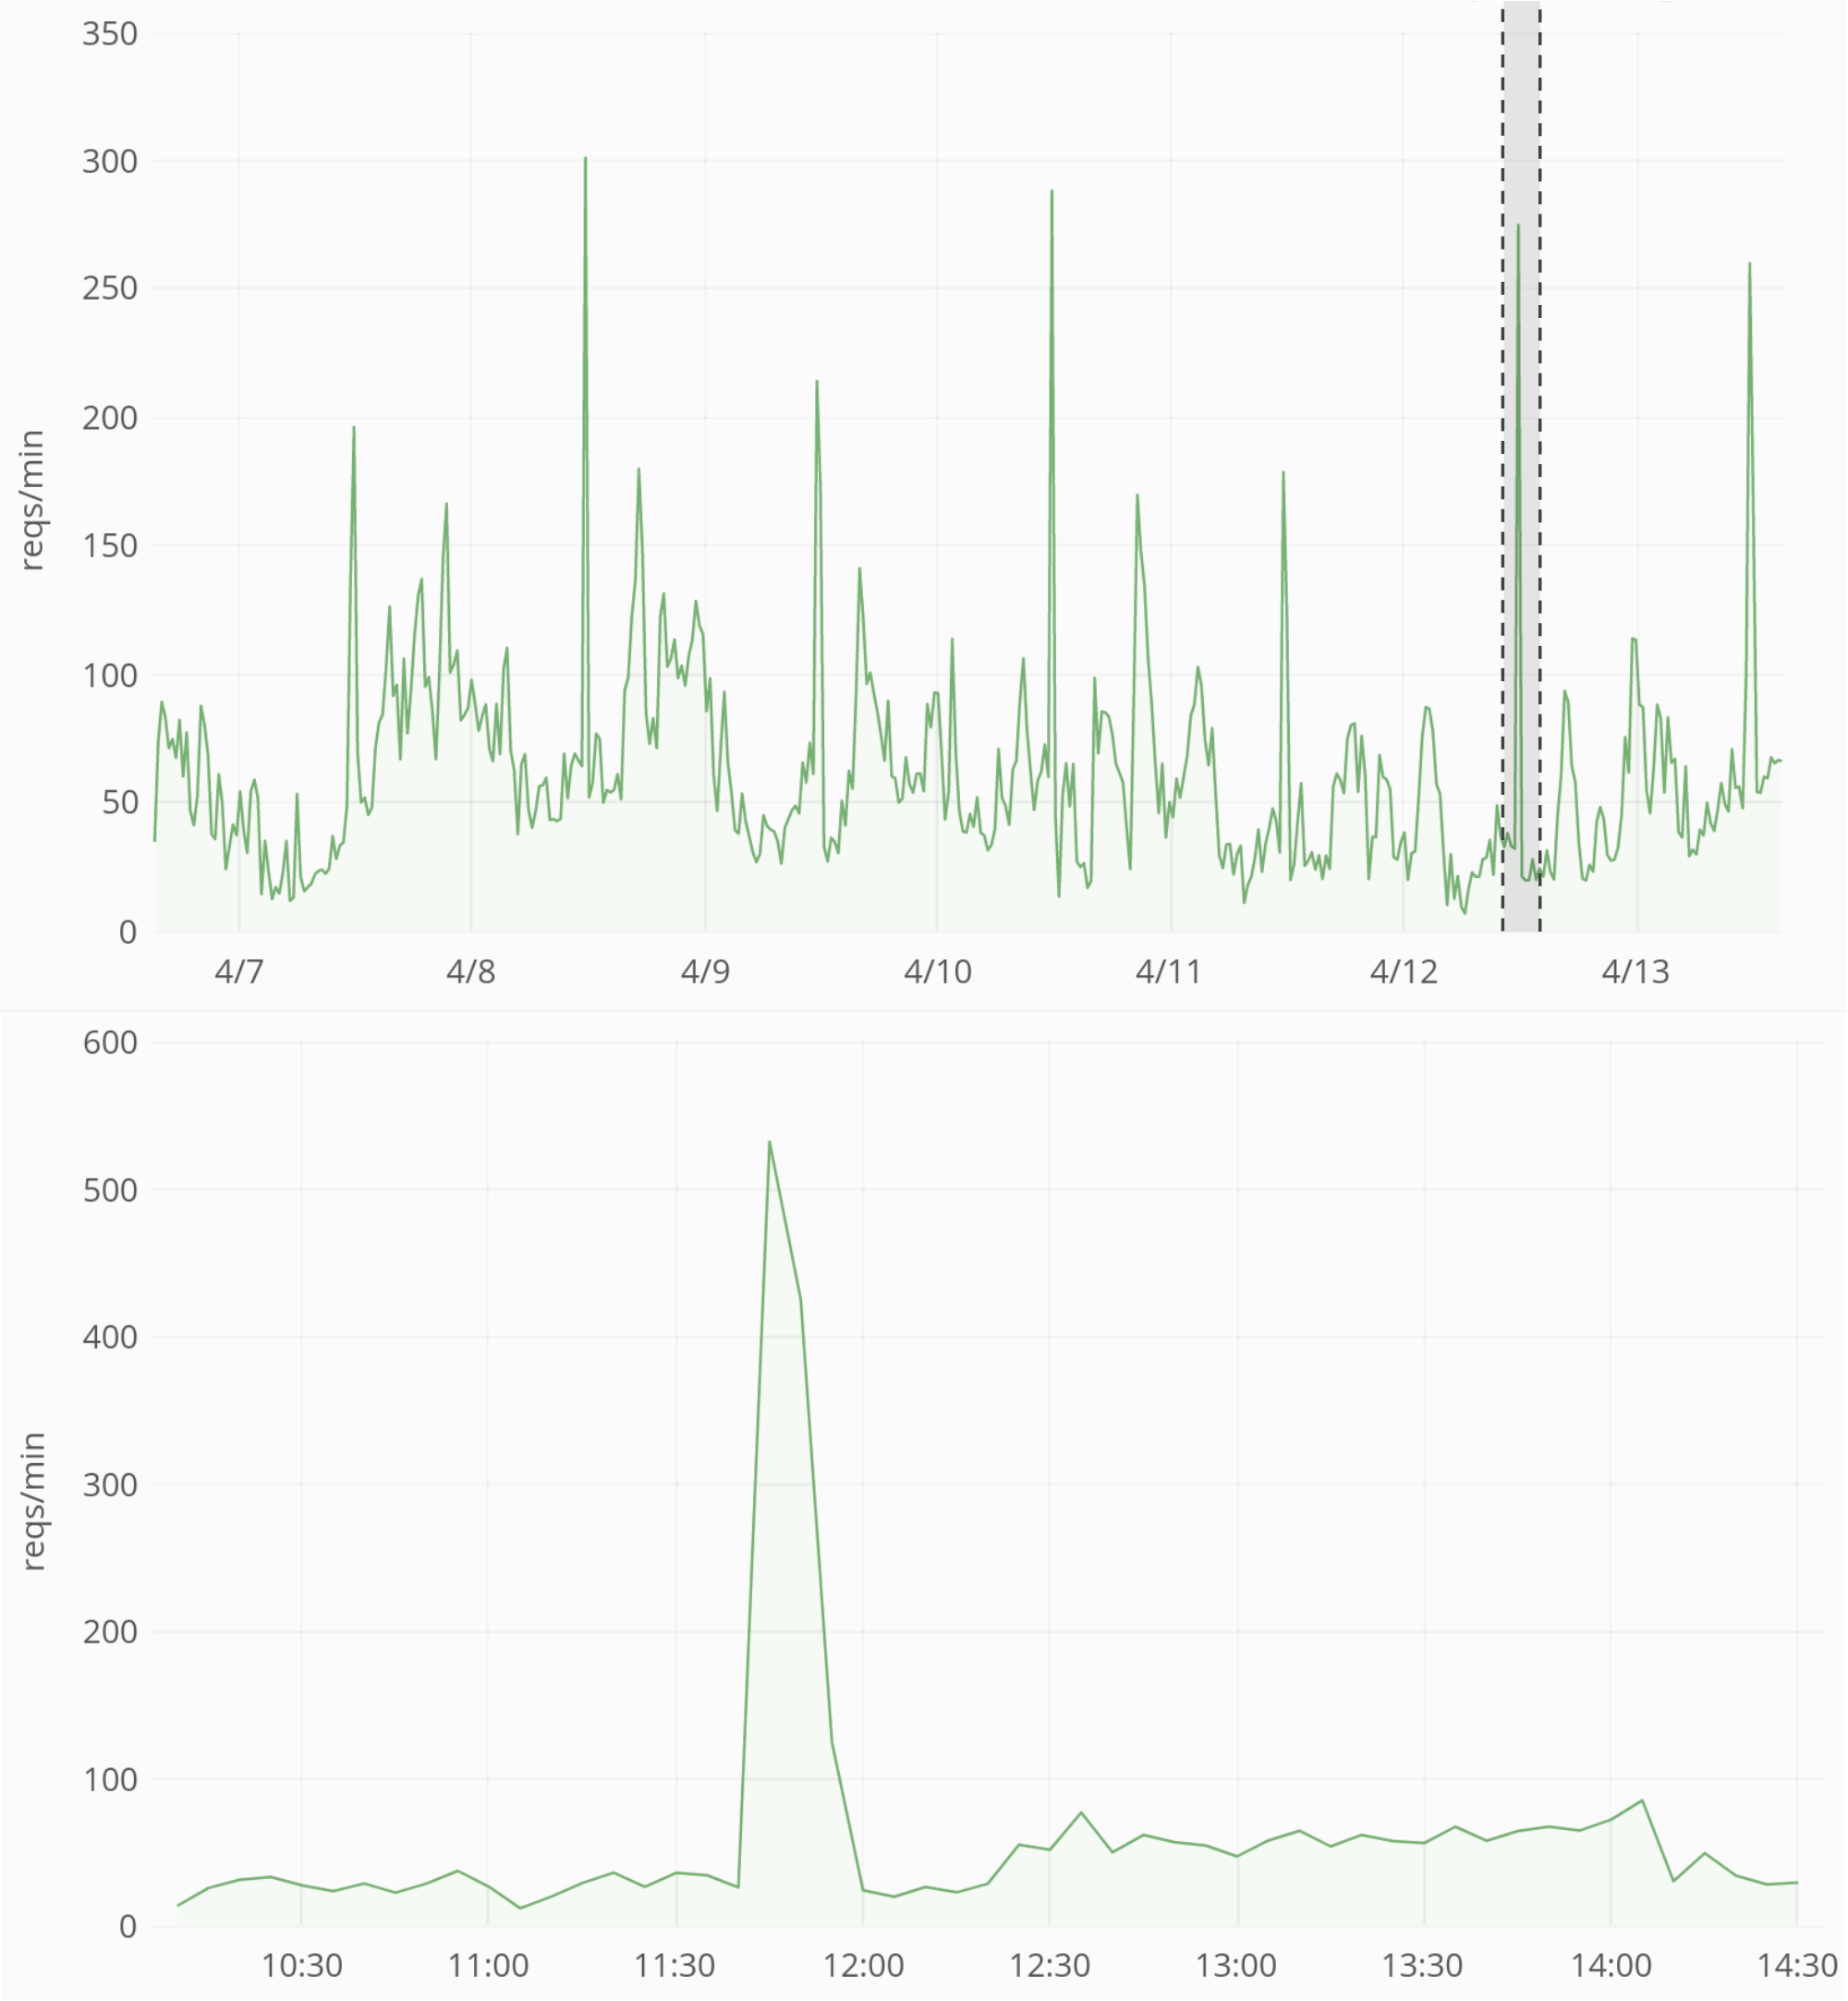
\includegraphics[width=.6\textwidth]{figures/ORES_request_activity_201804_week_vs_4hours}
  \caption{External requests per minute with a 4 hour block broken out to highlight a sudden burst of requests.}
  \label{fig:ores_request_rate}
\end{subfigure}\\
\begin{subfigure}[t]{\columnwidth}
  \centering
  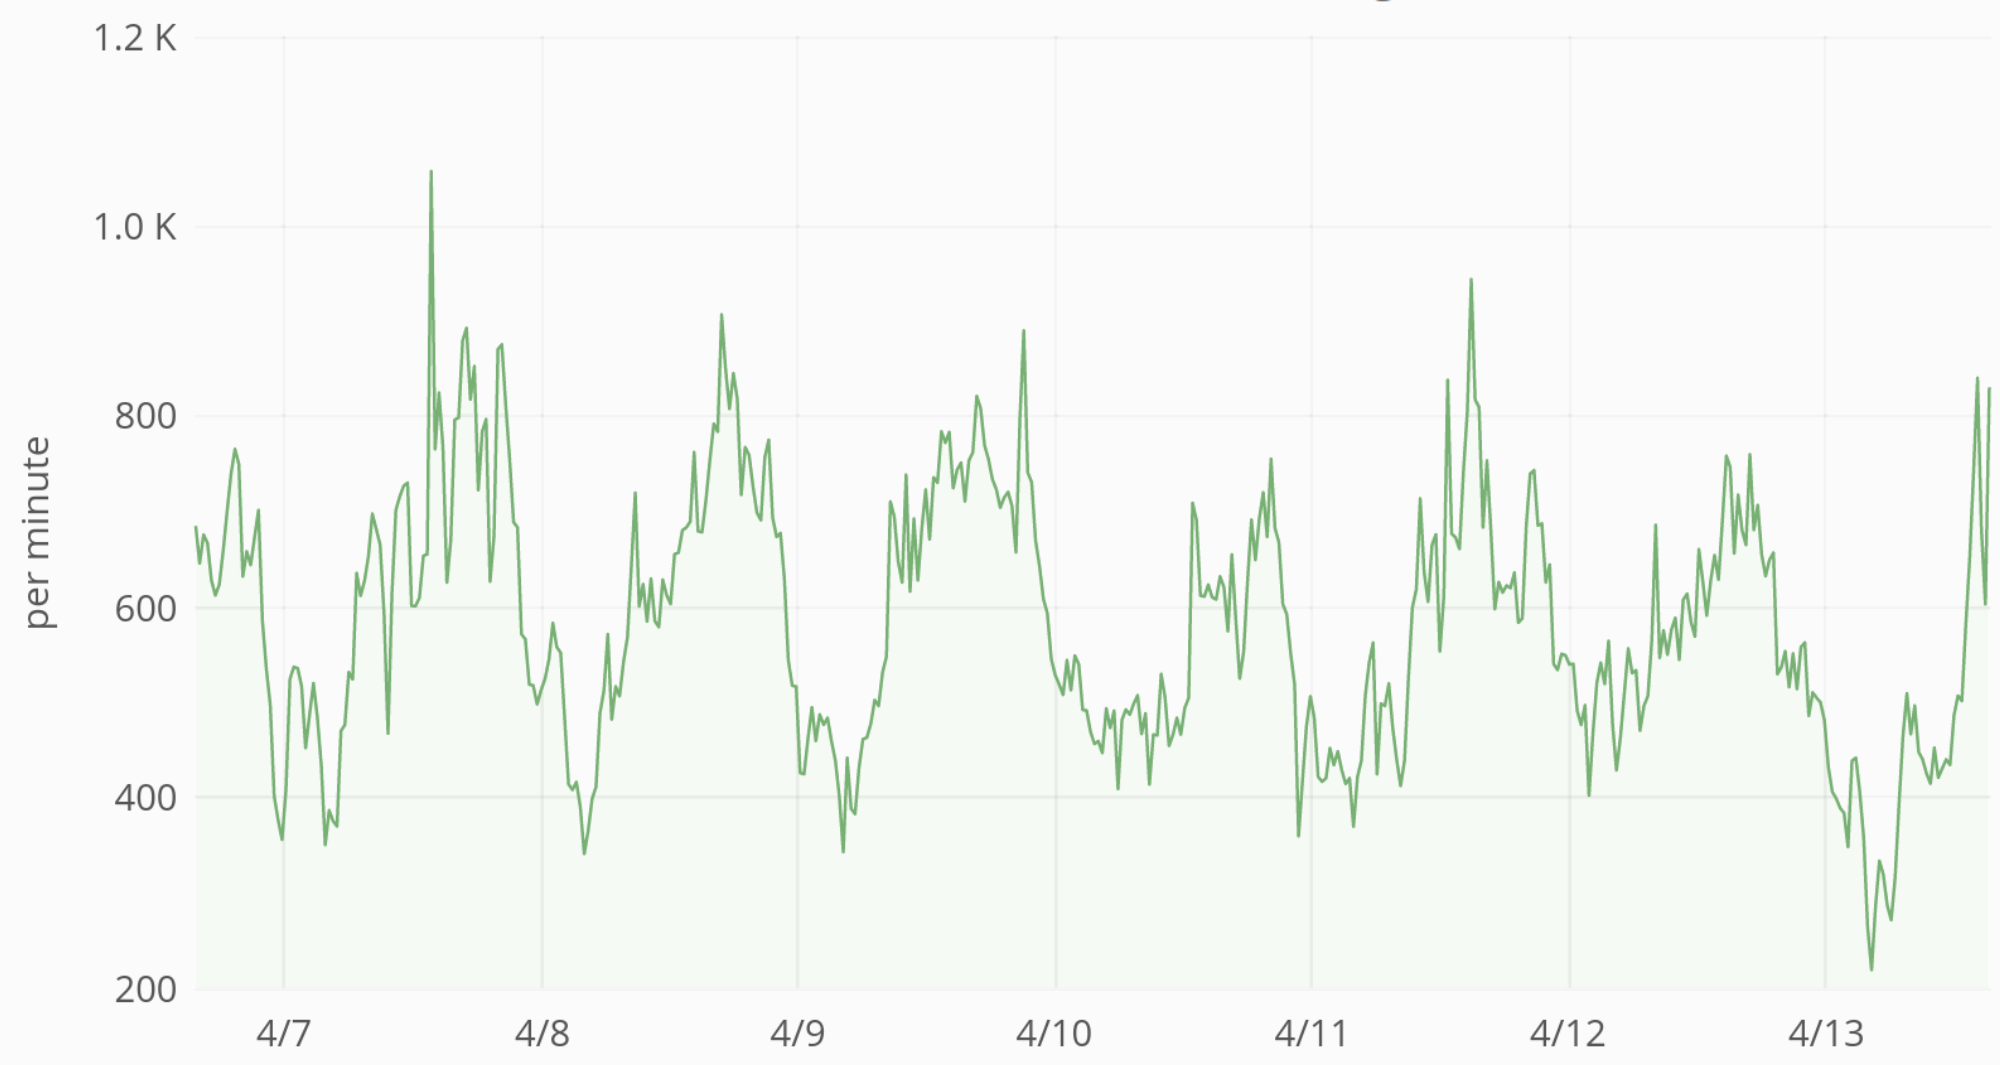
\includegraphics[width=.6\textwidth]{figures/ORES_precache_request_rate_201804}
  \caption{Precaching requests per minute}
  \label{fig:ores_precache_rate}
\end{subfigure}
\caption{Request rates to the ORES service for the week ending on April 13th, 2018}
\label{fig:ores_activity}
\end{figure*}


The ORES service has been online since July 2015\cite{halfaker2015artificial}.  Since then, usage has steadily risen as we've develop and deploy new models, and additional integrations are made by tool developers and researchers.  Currently, ORES supports 78 different models and 37 different language-specific wikis.

Generally, we see 50 to 125 requests per minute from external tools that are using ORES' predictions (excluding the MediaWiki extension that is more difficult to track).  Sometimes these external requests will burst up to 400-500 requests per second.  Figure~\ref{fig:ores_request_rate} shows the periodic and bursty nature of scoring requests received by the ORES service.  Note that every day at about 11:40 UTC, the request rate jumps---most likely a batch scoring job such as a bot.

Figure~\ref{fig:ores_precache_rate} shows our rate of precaching requests coming from our own systems.  This graph roughly reflects the rate of edits that are happening to all of the wikis that we support since we'll start a scoring job for nearly every edit as it happens.  Note that the number of precaching requests is about an order of magnitude higher than our known external score request rate.  This is expected, since Wikipedia editors and the tools they use will not request a score for every single revision.  This is a computational price we pay to attain a high cache hit rate and to ensure that our users get the quickest possible response for the scores that they \emph{do} need.

Taken together these strategies allow us to optimize the real-time quality control workflows and batch processing jobs of Wikipedians and their tools.  Without serious effort to make sure that ORES is practically fast and highly available to real-time use cases, ORES would become irrelevant to the target audience and thus irrelevant as a work-support infrastructure.  By engineering a system that conforms to the work-process needs of Wikipedians and their tools, we've built and systems intervention that has the potential gain wide adoption in Wikipedia's technical ecology.
